\documentclass[12pt,letterpaper, onecolumn]{exam}
\usepackage{amsmath}
\usepackage{pdfpages}
\usepackage{amssymb}
\usepackage{graphicx}
\usepackage{setspace}
\usepackage{nicefrac}
\usepackage{hyperref}
\setcounter{MaxMatrixCols}{20}
\usepackage[lmargin=71pt, tmargin=1.2in]{geometry}  %For centering solution box

\lhead{Principles of Navigation}
\rhead{Noah Miller}
\thispagestyle{empty}   %For removing header/footer from page 1


\begin{document}

\begingroup
\centering
\LARGE Principles of Navigation\\
\LARGE Homework 3 \\[0.5em]
\large \today\\[0.5em]
\large Noah Miller\par
\large 903949330\par
\large MECH 6970\par
\endgroup
\pointsdroppedatright   %Self-explanatory
\printanswers
\renewcommand{\solution}{\noindent\textbf{Answer:}\enspace}   %Replace "Ans:" with starting keyword in solution box



\begin{questions}
    \question{How many muiltiplies and additions are needed for each of the following computations?}
    \begin{parts}
        \part{Composition of rotations via rotation matrices, $\mathbf{C}_2^1\mathbf{C}_1^0$}

        \solution{%
            If we understand the rotation matrices to be in their most fundamental form, we can determine the number of multiplications and additions need to solve for $\mathbf{C}^0_2$. We start by defining both $\mathbf{C}_2^1$ and $\mathbf{C}_1^0$ which is a set of dot products between the respective frames.

            \begin{equation}
                \begin{split}
                    \mathbf{C}_2^1 & =
                    \begin{bmatrix}
                        x_2 \cdot x_1 & y_2 \cdot x_1 & z_2 \cdot x_1 \\
                        x_2 \cdot y_1 & y_2 \cdot y_1 & z_2 \cdot y_1 \\
                        x_2 \cdot z_1 & y_2 \cdot z_1 & z_2 \cdot z_1 \\
                    \end{bmatrix}
                \end{split}
                \label{eq:1}
            \end{equation}

            \begin{equation}
                \begin{split}
                    \mathbf{C}_1^0 & =
                    \begin{bmatrix}
                        x_1 \cdot x_0 & y_1 \cdot x_0 & z_1 \cdot x_0 \\
                        x_1 \cdot y_0 & y_1 \cdot y_0 & z_1 \cdot y_0 \\
                        x_1 \cdot z_0 & y_1 \cdot z_0 & z_1 \cdot z_0 \\
                    \end{bmatrix}
                \end{split}
                \label{eq:2}
            \end{equation}

            Defining these two rotations matrices we see that there 9 multiplications for each, so we add those to our running tally.
            Next, we multiply these together, which is a combination of multiplication and addition.
            \begin{equation}
                \begin{split}
                    \mathbf{C}_2^1\mathbf{C}_1^0 & =
                    \begin{bmatrix}
                        x_2 \cdot x_1 & y_2 \cdot x_1 & z_2 \cdot x_1 \\
                        x_2 \cdot y_1 & y_2 \cdot y_1 & z_2 \cdot y_1 \\
                        x_2 \cdot z_1 & y_2 \cdot z_1 & z_2 \cdot z_1 \\
                    \end{bmatrix}
                    \begin{bmatrix}
                        x_1 \cdot x_0 & y_1 \cdot x_0 & z_1 \cdot x_0 \\
                        x_1 \cdot y_0 & y_1 \cdot y_0 & z_1 \cdot y_0 \\
                        x_1 \cdot z_0 & y_1 \cdot z_0 & z_1 \cdot z_0 \\
                    \end{bmatrix} \\
                    \mathbf{C}_2^1\mathbf{C}_1^0 (:,1) & =
                    \begin{bmatrix}
                        \mathbf{C}_2^1(1,1)\mathbf{C}_1^0(1,1) + \mathbf{C}_2^1(1,2)\mathbf{C}_1^0(2,1) + \mathbf{C}_2^1(1,3)\mathbf{C}_1^0(3,1) \\
                        \mathbf{C}_2^1(2,1)\mathbf{C}_1^0(1,1) + \mathbf{C}_2^1(2,2)\mathbf{C}_1^0(2,1) + \mathbf{C}_2^1(2,3)\mathbf{C}_1^0(3,1) \\
                        \mathbf{C}_2^1(3,1)\mathbf{C}_1^0(1,1) + \mathbf{C}_2^1(3,2)\mathbf{C}_1^0(2,1) + \mathbf{C}_2^1(3,3)\mathbf{C}_1^0(3,1) \\
                    \end{bmatrix}
                \end{split}
                \label{eq:3}
            \end{equation}

            For the first column of matrix multiplication, there are 9 multiplications and 6 additions. We can triple this to account for the other two columns to add to our running tally.

            Adding our running total together, for part \ref{part@1@1}, we see there is 45 multiplications and 18 additions.
        }

        \part{Composition of rotations via quaternions, $\bar{q}_1^{\;2} \otimes \bar{q}_0^{\;1}$}

        \solution{%
            Counting the number of multiplications and additions of the tensor product between two quaternions is done easily if we layout the multiplication in its fundamental form.
            \begin{equation}
                \begin{split}
                    \bar{q}_1^{\;2} \otimes \bar{q}_0^{\;1} & =
                    \begin{bmatrix}
                        q_1^{2}(1) & -q_1^{2}(2) & -q_1^{2}(3) & -q_1^{2}(4) \\
                        q_1^{2}(2) & q_1^{2}(1)  & -q_1^{2}(4) & q_1^{2}(3)  \\
                        q_1^{2}(3) & q_1^{2}(4)  & q_1^{2}(1)  & q_1^{2}(2)  \\
                        q_1^{2}(4) & -q_1^{2}(3) & -q_1^{2}(2) & q_1^{2}(1)  \\
                    \end{bmatrix}
                    \begin{bmatrix}
                        q_0^{1}(1) \\
                        q_0^{1}(2) \\
                        q_0^{1}(3) \\
                        q_0^{1}(4) \\
                    \end{bmatrix}\\
                    \bar{q}_1^{\;2} \otimes \bar{q}_0^{\;1} & =
                    \begin{bmatrix}
                        q_1^{2}(1)q_0^{1}(1) + -q_1^{2}(2)q_0^{1}(2) + -q_1^{2}(3)q_0^{1}(3) + -q_1^{2}(4)q_0^{1}(4) \\
                        q_1^{2}(2)q_0^{1}(1) + q_1^{2}(1)q_0^{1}(2) + -q_1^{2}(4)q_0^{1}(3) + q_1^{2}(3)q_0^{1}(4)   \\
                        q_1^{2}(3)q_0^{1}(1) + q_1^{2}(4)q_0^{1}(2) + q_1^{2}(1)q_0^{1}(3) + q_1^{2}(2)q_0^{1}(4)    \\
                        q_1^{2}(4)q_0^{1}(1) + -q_1^{2}(3)q_0^{1}(2) + -q_1^{2}(2)q_0^{1}(3) + q_1^{2}(1)q_0^{1}(4)  \\
                    \end{bmatrix}
                \end{split}
                \label{eq:4}
            \end{equation}

            From here, we see a total of 16 multiplications and 12 additions.
        }

        \part{Recoordinatization of a vector via rotation matrix, $\mathbf{C}_2^1\vec{r}^{\;1}$}

        \solution{%
            From part \ref{part@1@1} we know the formation of $\mathbf{C}_2^1$ contains 9 multiplications. So now we just have to count the number of multiplications and additions that occur when evaluating $\mathbf{C}_2^1\vec{r}^{\;1}$.

            \begin{equation}
                \begin{split}
                    \mathbf{C}_2^1\vec{r}^{\;1} & =
                    \begin{bmatrix}
                        x_2 \cdot x_1 & y_2 \cdot x_1 & z_2 \cdot x_1 \\
                        x_2 \cdot y_1 & y_2 \cdot y_1 & z_2 \cdot y_1 \\
                        x_2 \cdot z_1 & y_2 \cdot z_1 & z_2 \cdot z_1 \\
                    \end{bmatrix}
                    \begin{bmatrix}
                        r_x^1 \\
                        r_y^1 \\
                        r_z^1 \\
                    \end{bmatrix}\\
                    \mathbf{C}_2^1\vec{r}^{\;1} & =
                    \begin{bmatrix}
                        \mathbf{C}_2^1(1,1)r_x^1 + \mathbf{C}_2^1(1,2)r_y^1 + \mathbf{C}_2^1(1,3)r_z^1 \\
                        \mathbf{C}_2^1(2,1)r_x^1 + \mathbf{C}_2^1(2,2)r_y^1 + \mathbf{C}_2^1(2,3)r_z^1 \\
                        \mathbf{C}_2^1(3,1)r_x^1 + \mathbf{C}_2^1(3,2)r_y^1 + \mathbf{C}_2^1(3,3)r_z^1 \\
                    \end{bmatrix}\\
                \end{split}
                \label{eq:5}
            \end{equation}
            From Equation \ref{eq:5} we see a total of 6 additions and 18 multiplications.
        }

        \part{Recoordinatization of a vector via quaternion, $\bar{q}_1^{\;2} \otimes \breve{r}^1 \otimes \left(\bar{q}_1^{\;2}\right)^{-1}$}

        \solution{%
        To evaluate the recoordinatization of a vector with quaternions, $\bar{q}_1^{\;2} \otimes \breve{r}^1 \otimes \left(\bar{q}_1^{\;2}\right)^{-1}$, we should be able to double the amount of multiplications and additions seen from part \ref{part@1@2}. Doing this, we see that two tensor products require 32 multiplications and 24 additions.
        }
    \end{parts}
    \clearpage
    \question{Consider the three-link, planar robot shown below for which four coordinate frames have been assigned. Frame $\{0\}$ is fixed, frame $\{1\}$ rotates with angle $\theta_1$ relative to Frame $\{0\}$, frame $\{2\}$ rotates with $\theta_2$ relative to frame $\{1\}$, and frame $\{3\}$ translates with distance $d_3$ relative to frame $\{2\}$.

        \begin{figure*}[!h]
            \centering
            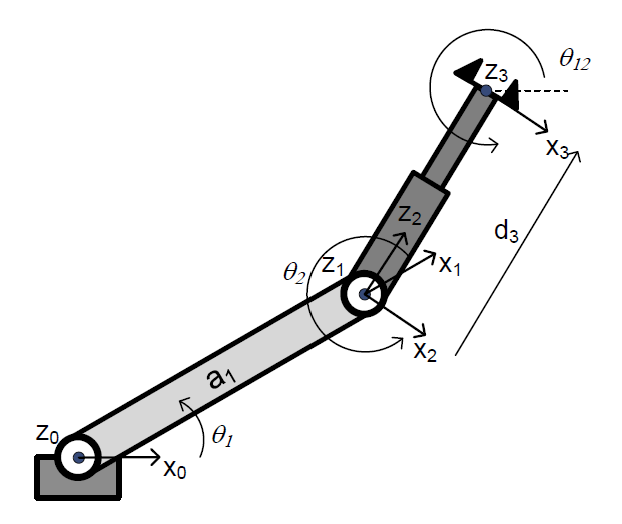
\includegraphics[width=0.5\linewidth]{Q2ps.png}
        \end{figure*}


        The rotation matrices and displacements between frames are shown below.

        \centering
        $\mathbf{C}_1^0 =
            \begin{bmatrix}
                cos(\theta_1) & -sin(\theta_1) & 0 \\
                sin(\theta_1) & cos(\theta_1)  & 0 \\
                0             & 0              & 1 \\
            \end{bmatrix}
        $,
        $\vec{r}^{\;0}_{01} =
            \begin{bmatrix}
                a_1cos(\theta_1) \\
                a_1sin(\theta_1) \\
                0                \\
            \end{bmatrix}
        $,
        $\mathbf{C}_2^1 =
            \begin{bmatrix}
                cos(\theta_2) & 0  & -sin(\theta_2) \\
                sin(\theta_2) & 0  & cos(\theta_2)  \\
                0             & -1 & 0              \\
            \end{bmatrix}
        $

        \qquad \qquad \qquad \qquad \quad
        $\vec{r}^{\;1}_{12} =
            \begin{bmatrix}
                0 \\
                0 \\
                0 \\
            \end{bmatrix}$
        $\mathbf{C}_2^3 =
            \begin{bmatrix}
                1 & 0 & 0  \\
                0 & 0 & -1 \\
                0 & 1 & 0  \\
            \end{bmatrix}
        $,\quad
        $\vec{r}^{\;2}_{23} =
            \begin{bmatrix}
                0   \\
                0   \\
                d_3 \\
            \end{bmatrix}
        $
    }
    \begin{parts}
        \part{Determine the rotation matrix $\mathbf{C}_3^0$.}

        \solution{%
            Determining $\mathbf{C}_3^0$ can be done by multiplying the 3 given rotation matrices in a specific order to reflect the angular relationships between frame \{0\} and frame \{3\}.

            \begin{equation}
                \begin{split}
                    \mathbf{C}_3^0 & = \mathbf{C}_1^0 \mathbf{C}_2^1 \mathbf{C}_3^2\\
                    \mathbf{C}_3^0 & =
                    \begin{bmatrix}
                        cos(\theta_1) & -sin(\theta_1) & 0 \\
                        sin(\theta_1) & cos(\theta_1)  & 0 \\
                        0             & 0              & 1 \\
                    \end{bmatrix}
                    \begin{bmatrix}
                        cos(\theta_2) & 0  & -sin(\theta_2) \\
                        sin(\theta_2) & 0  & cos(\theta_2)  \\
                        0             & -1 & 0              \\
                    \end{bmatrix}
                    \begin{bmatrix}
                        1 & 0 & 0  \\
                        0 & 0 & -1 \\
                        0 & 1 & 0  \\
                    \end{bmatrix}\\
                    \mathbf{C}_3^0 & =
                    \begin{bmatrix}
                        cos(\theta_1) & -sin(\theta_1) & 0 \\
                        sin(\theta_1) & cos(\theta_1)  & 0 \\
                        0             & 0              & 1 \\
                    \end{bmatrix}
                    \begin{bmatrix}
                        cos(\theta_2) & -sin(\theta_2) & 0 \\
                        sin(\theta_2) & cos(\theta_2)  & 0 \\
                        0             & 0              & 1 \\
                    \end{bmatrix} \\
                    \mathbf{C}_3^0 & =
                    \begin{bmatrix}
                        c\theta_1c\theta_2 - s\theta_1s\theta_2 & -\left(c\theta_1s\theta_2 + c\theta_2s\theta_1\right) & 0 \\
                        c\theta_1s\theta_2 + c\theta_2s\theta_1 & c\theta_1c\theta_2 - s\theta_1s\theta_2               & 0 \\
                        0                                       & 0                                                     & 1 \\
                    \end{bmatrix}
                \end{split}
                \label{}
            \end{equation}
        }
        \part{Determine the translation vector $\vec{r}^{\;0}_{03}$}

        \solution{%
            From class we learned that vectors must be in the same frame to add them together. We can do this by using rotation matrices to transform the vectors to the same frame.

            \begin{equation}
                \begin{split}
                    \vec{r}^{\;0}_{03} & = \vec{r}^{\;0}_{01} + \mathbf{C}_1^0 \vec{r}^{\;1}_{12} + \mathbf{C}_1^0 \mathbf{C}_2^1 \vec{r}^{\;2}_{23}\\
                    \vec{r}^{\;0}_{03} & = \left[\begin{array}{c} a_{1}\,\cos\left(\theta_1\right)-d_{3}\,\left(\cos\left(\theta_1\right)\,\sin\left(\theta_2\right)+\cos\left(\theta_2\right)\,\sin\left(\theta_1\right)\right)\\ d_{3}\,\left(\cos\left(\theta_1\right)\,\cos\left(\theta_2\right)-\sin\left(\theta_1\right)\,\sin\left(\theta_2\right)\right)+a_{1}\,\sin\left(\theta_1\right)\\ 0 \end{array}\right]\\
                \end{split}
                \label{eq:7}
            \end{equation}
        }

        \part{Determine the following angular velocities as skew-symmetric matrices $\tilde{\omega}$ and vectors $\vec{\omega}$. Note $\theta_1$,$\theta_2$, and $d_3$ can vary with time.}
        \begin{subparts}
            \subpart{$\tilde{\omega}^0_{01}$, $\vec{\omega}^0_{01}$}

            \solution{%
            \begin{equation}
                \begin{split}
                    \tilde{\omega}^0_{01} & = \dot{\mathbf{C}}_1^0\left(\mathbf{C}_1^0\right)^{-1}\\
                    \tilde{\omega}^0_{01} & =
                    \begin{bmatrix}
                        -\dot{\theta_1}\sin\theta_1 & -\dot{\theta_1}\cos\theta_1 & 0 \\
                        \dot{\theta_1}\cos\theta_1  & -\dot{\theta_1}\sin\theta_1 & 0 \\
                        0                           & 0                           & 0 \\
                    \end{bmatrix}
                    \left(
                    \begin{bmatrix}
                        cos(\theta_1) & -sin(\theta_1) & 0 \\
                        sin(\theta_1) & cos(\theta_1)  & 0 \\
                        0             & 0              & 1 \\
                    \end{bmatrix}
                    \right)^{-1}\\
                \end{split}
                \label{}
            \end{equation}
            \[\tilde{\omega}^0_{01} = \left[\begin{array}{ccc} 0 & -\dot{\theta}_1 & 0\\ \dot{\theta}_1 & 0 & 0\\ 0 & 0 & 0 \end{array}\right]\]
            \[\vec{\omega}^0_{01} = \begin{bmatrix}
                    0              \\
                    0              \\
                    \dot{\theta}_1 \\
                \end{bmatrix} \]
            }
            \subpart{$\tilde{\omega}^1_{12}$, $\vec{\omega}^1_{12}$}

            \solution{%
            \begin{equation}
                \begin{split}
                    \tilde{\omega}^1_{12} & = \dot{\mathbf{C}}_2^1\left(\mathbf{C}_2^1\right)^{-1}\\
                    \tilde{\omega}^1_{12} & =
                    \begin{bmatrix}
                        -\dot{\theta_2}\sin\theta_2 & 0 & -\dot{\theta_2}\cos\theta_2 \\
                        \dot{\theta_2}\cos\theta_2  & 0 & -\dot{\theta_2}\sin\theta_2 \\
                        0                           & 0 & 0                           \\
                    \end{bmatrix}
                    \left(
                    \begin{bmatrix}
                        cos(\theta_2) & 0  & -sin(\theta_2) \\
                        sin(\theta_2) & 0  & cos(\theta_2)  \\
                        0             & -1 & 0              \\
                    \end{bmatrix}
                    \right)^{-1}\\
                \end{split}
                \label{}
            \end{equation}
            \[\tilde{\omega}^1_{12} = \left[\begin{array}{ccc} 0 & -\dot{\theta}_2 & 0\\ \dot{\theta}_2 & 0 & 0\\ 0 & 0 & 0 \end{array}\right]\]
            \[\vec{\omega}^1_{12} = \begin{bmatrix}
                    0              \\
                    0              \\
                    \dot{\theta}_2 \\
                \end{bmatrix} \]}
            \subpart{$\tilde{\omega}^2_{23}$, $\vec{\omega}^2_{23}$}

            \solution{%
            Using Equation \ref{eq:6}, we can find $\tilde{\omega}^2_{23}$ and then transform it to $\vec{\omega}^2_{23}$.
            \begin{equation}
                \begin{split}
                    \tilde{\omega}^2_{23} & = \dot{\mathbf{C}}_2^3 \left(\mathbf{C}_2^3\right)^{-1}\\
                    \tilde{\omega}^2_{23} & =
                    \begin{bmatrix}
                        0 & 0 & 0 \\
                        0 & 0 & 0 \\
                        0 & 0 & 0 \\
                    \end{bmatrix}\left(
                    \begin{bmatrix}
                        1 & 0  & 0 \\
                        0 & 0  & 1 \\
                        0 & -1 & 0 \\
                    \end{bmatrix}\right)^{-1}\\
                    \tilde{\omega}^2_{23} & =
                    \begin{bmatrix}
                        0 & 0 & 0 \\
                        0 & 0 & 0 \\
                        0 & 0 & 0 \\
                    \end{bmatrix}\\
                    \vec{\omega}^2_{23} & =
                    \begin{bmatrix}
                        0 \\
                        0 \\
                        0 \\
                    \end{bmatrix}\\
                \end{split}
                \label{eq:6}
            \end{equation}
            }

            \subpart{$\tilde{\omega}^0_{03}$, $\vec{\omega}^0_{03}$}

            \solution{%
                Just like adding position vectors together ($\mathbf{r_{03}^0}$), angular rates to be added together must be in the same frame. We can do this setting up the fundamental equation of the angular rates for each frame and then deriving each one to get our final answer.

                \begin{equation}
                    \begin{split}
                        \tilde{\omega}^0_{03} & = \tilde{\omega}^0_{01} + \tilde{\omega}^0_{12} + \tilde{\omega}^0_{23}\\
                        \tilde{\omega}^0_{03} & = \tilde{\omega}^0_{01} + \mathbf{C}^0_1\tilde{\omega}^1_{12} + \mathbf{C}^0_1\mathbf{C}^1_2\tilde{\omega}^2_{23}\\
                        \tilde{\omega}^0_{03} & =
                        \begin{bmatrix}
                            0              & -\dot{\theta}_1 & 0 \\
                            \dot{\theta}_1 & 0               & 0 \\
                            0              & 0               & 0 \\
                        \end{bmatrix} +
                        \begin{bmatrix}
                            cos(\theta_1) & -sin(\theta_1) & 0 \\
                            sin(\theta_1) & cos(\theta_1)  & 0 \\
                            0             & 0              & 1 \\
                        \end{bmatrix}
                        \begin{bmatrix}
                            0              & -\dot{\theta}_2 & 0 \\
                            \dot{\theta}_2 & 0               & 0 \\
                            0              & 0               & 0 \\
                        \end{bmatrix}\\
                        + &
                        \begin{bmatrix}
                            cos(\theta_1) & -sin(\theta_1) & 0 \\
                            sin(\theta_1) & cos(\theta_1)  & 0 \\
                            0             & 0              & 1 \\
                        \end{bmatrix}
                        \begin{bmatrix}
                            cos(\theta_2) & 0  & -sin(\theta_2) \\
                            sin(\theta_2) & 0  & cos(\theta_2)  \\
                            0             & -1 & 0              \\
                        \end{bmatrix}
                        \begin{bmatrix}
                            0 & 0 & 0 \\
                            0 & 0 & 0 \\
                            0 & 0 & 0 \\
                        \end{bmatrix}\\
                        \tilde{\omega}^0_{03} & =
                        \begin{bmatrix}
                            0                     & -(\theta_1 + \theta_2) & 0 \\
                            (\theta_1 + \theta_2) & 0                      & 0 \\
                            0                     & 0                      & 0 \\
                        \end{bmatrix}\\
                        \vec{\omega}^0_{03} & =
                        \begin{bmatrix}
                            0                     \\
                            0                     \\
                            (\theta_1 + \theta_2) \\
                        \end{bmatrix}\\
                    \end{split}
                    \label{}
                \end{equation}
            }
        \end{subparts}

    \end{parts}
    \clearpage
    \question{Consider the time-varying coordinate transformation matrix $\mathbf{C}^{n}_{b}$ given below that describes the orientation of the body frame as it rotates with respect to the navigation frame.
        \[\mathbf{C}^n_b =
            \begin{bmatrix}
                cos(t)  & sin(t)sin(t^2)  & sin(t)cos(t^2) \\
                0       & cos(t^2)        & -sin(t^2)      \\
                -sin(t) & cos(t) sin(t^2) & cos(t)cos(t^2) \\
            \end{bmatrix} \]
    }
    \begin{parts}
        \part{Compute expressions for $\psi$,$\theta$, and $\phi$ based on fixed-axis definition of roll, pitch, yaw assuming a 1,2,3 series of rotations (roll,pitch,yaw).}

        \solution{%
            From class, we determined the Euler angles to be
            \begin{equation}
                \begin{split}
                    \phi & = tan^{-1}\left(\frac{-C_{23}}{C_{33}}\right) \\
                    \theta & = sin^{-1}(-C_{13})\\
                    \psi & = tan^{-1}\left(\frac{-C_{12}}{C_{11}}\right)\\
                \end{split}
                \label{eulerAngles}
            \end{equation}
        }

        \part{Use MATLAB to plot $\psi$,$\theta$, and $\phi$ as a function of time.}

        The simulation was run for 10 seconds with a sampling rate of 100 Hertz.

        \begin{figure}[!h]
            \centering
            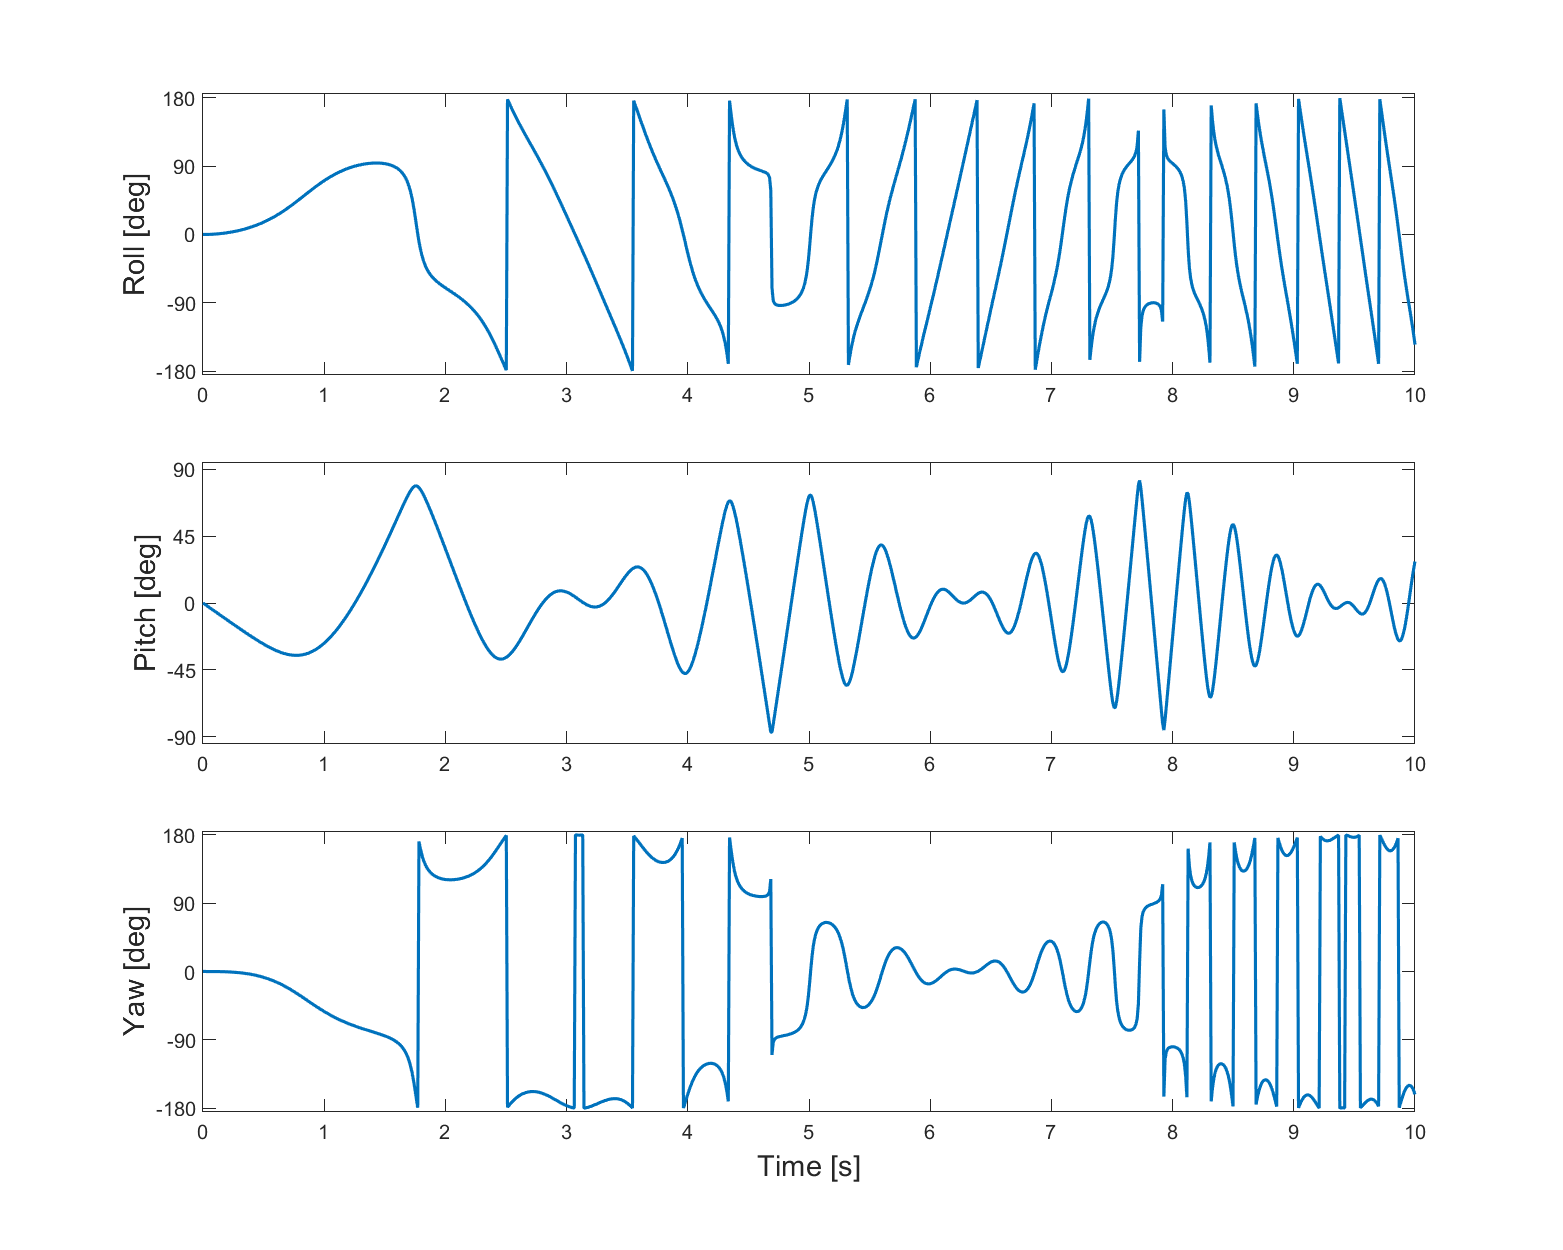
\includegraphics[width=0.8\linewidth]{Euler_Angles.png}
            \caption{Roll, Pitch, and Yaw angles plotted as a function of time.}
            \label{fig:euler}
        \end{figure}

    \end{parts}
    \clearpage
    \question{Consider the time-varying coordinate transformation matrix $\mathbf{C}^n_b$ give below that describe the orientation of the body as it rotates with respect to the navigation frame.
        \[\mathbf{C}^n_b =
            \begin{bmatrix}
                cos(t)  & sin(t)sin(t^2)  & sin(t)cos(t^2) \\
                0       & cos(t^2)        & -sin(t^2)      \\
                -sin(t) & cos(t) sin(t^2) & cos(t)cos(t^2) \\
            \end{bmatrix} \]
    }
    \begin{parts}
        \part{Determine the analytic form of the time-derivative of $\mathbf{C}^n_b$ (i.e. $\dot{\mathbf{C}}^n_b = \frac{d\mathbf{C}^n_b}{dt}$) via a term-by-term differentiation.}

        We can use the \textit{Symbolic Math Toolbox} to differentiate the matrix for us very easily. Using \textit{diff} in MATLAB produces
        \[\dot{\mathbf{C}}^n_b = \left[\begin{array}{ccc} -s\left(t\right) & s\left(t^2\right)c\left(t\right)+2t\cdot c\left(t^2\right)s\left(t\right) & c\left(t^2\right)c\left(t\right)-2t\cdot s\left(t^2\right)s\left(t\right)\\ 0 & -2t\cdot s\left(t^2\right) & -2t\cdot c\left(t^2\right)\\ -c\left(t\right) & 2t\cdot c\left(t^2\right)c\left(t\right)-s\left(t^2\right)s\left(t\right) & -c\left(t^2\right)s\left(t\right)-2t\cdot s\left(t^2\right)c\left(t\right) \end{array}\right]\]



        \part{Develop MATLAB functions which accept $t$ (i.e time) as a numerical input and return $\mathbf{C}^n_b$ and $\dot{\mathbf{C}}^n_b$, respectively, as numerical outputs.}

        \solution{%
            The created function is appended at the end of this submission.
        }

        \part{Using the $\mathbf{C}^n_b$ and $\dot{\mathbf{C}}^n_b$ functions from above, compute the angular velocity vector $\vec{\omega}^{\;n}_{nb}$ at time $t = 0$ seconds. (HINT: You might want to compute $\tilde{\omega}^{n}_{nb}$)}

        \solution{%
            For the following parts we can solve for $\vec{\omega}^{\;n}_{nb}$ using the following equation.
            \[\dot{\mathbf{C}}^n_b(\mathbf{C}^n_b)^{-1} = \tilde{\omega}^{\;n}_{nb} \]
            If we understand that $\tilde{\omega}^{\;n}_{nb}$ is just the skew-symmetric form of $\vec{\omega}^{\;n}_{nb}$, we can go between forms quite easily with Equation \ref{eq:10}.
            \begin{equation}
                \begin{split}
                    \tilde{\omega}^{\;n}_{nb} & =
                    \begin{bmatrix}
                        0         & -\omega_z & \omega_y  \\
                        \omega_z  & 0         & -\omega_x \\
                        -\omega_y & \omega_x  & 0         \\
                    \end{bmatrix}\\
                    \vec{\omega}^{\;n}_{nb} & =
                    \begin{bmatrix}
                        \omega_x \\
                        \omega_y \\
                        \omega_z \\
                    \end{bmatrix}\\
                \end{split}
                \label{eq:10}
            \end{equation}

            Using the aforementioned equations, we find that $\vec{\omega}^{\;n}_{nb}$ at time $t = 0$ seconds is
            \[\vec{\omega}^{\;n}_{nb}\vert_{(t = 0)}  =
                \begin{bmatrix}
                    0 \\
                    1 \\
                    0 \\
                \end{bmatrix} \]
        }
        \begin{subparts}
            \subpart{What is the magnitude (i.e. $\dot{\theta}$,angular speed) of the angular velocity?}

            \solution{%
                We can find the magnitude of $\vec{\omega}^{\;n}_{nb}\vert_{(t = 0)}$ by using \textit{norm} in MATLAB.
                \begin{equation}
                    \begin{split}
                        norm(\vec{\omega}^{\;n}_{nb}\vert_{(t = 0)}) & = 1
                    \end{split}
                    \label{eq:11}
                \end{equation}
            }

            \subpart{About what unit vector ($\vec{k}^{\;n}_{nb}$) has the instantaneous rotation occurred?}

            \solution{%
                We can find the unit vector, $\vec{k}^{\;n}_{nb}$, by first finding $\theta$. This can be done by using $\mathbf{C}^n_b$ evaluated at time $t = 0$ seconds.

                \begin{equation}
                    \begin{split}
                        \theta & = \cos^{-1}\left(\frac{trace(\mathbf{C}^n_b) - 1}{2} \right)\\
                        \theta & = 0^o \\
                    \end{split}
                    \label{eq:12}
                \end{equation}

                Then, using $\theta$ we can solve for the unit vector that the body is rotating about.
                \begin{equation}
                    \begin{split}
                        \vec{k}^{\;n}_{nb} & =
                        \begin{bmatrix}
                            \mathbf{C}^n_b(3,2) - \mathbf{C}^n_b(2,3) \\
                            \mathbf{C}^n_b(1,3) - \mathbf{C}^n_b(3,1) \\
                            \mathbf{C}^n_b(2,1) - \mathbf{C}^n_b(1,2) \\
                        \end{bmatrix}\frac{1}{2\sin\theta}
                    \end{split}
                    \label{eq:13}
                \end{equation}

                When doing this for time $t = 0$ seconds, we see that $\theta$ is 0, thus giving us an undefined unit vector. This is to be expected because the body did not have any initial angular velocity.
            }
        \end{subparts}

        \part{Using the $\mathbf{C}^n_b$ and $\dot{\mathbf{C}}^n_b$ functions from above, compute the angular velocity vector $\vec{\omega}^{\;n}_{nb}$ at time $t = 0.5$ seconds.}
        \[\vec{\omega}^{\;n}_{nb}\vert_{(t = 0.5)}  =
            \begin{bmatrix}
                0.8776  \\
                1       \\
                -0.4794 \\
            \end{bmatrix} \]
        \begin{subparts}
            \subpart{What is the magnitude (i.e. $\dot{\theta}$,angular speed) of the angular velocity?}
            \begin{equation}
                \begin{split}
                    \dot{\theta} & = 1.4142\left[\frac{deg}{s}\right] \\
                \end{split}
            \end{equation}
            \subpart{About what unit vector ($\vec{k}^{\;n}_{nb}$) has the instantaneous rotation occurred?}
            \begin{equation}
                \begin{split}
                    \vec{k}^{\;n}_{nb} & =
                    \begin{bmatrix}
                        0.43876        \\
                        0.89159        \\
                        -      0.11203 \\
                    \end{bmatrix}
                \end{split}
            \end{equation}
        \end{subparts}
        \clearpage
        \part{Using the $\mathbf{C}^n_b$ and $\dot{\mathbf{C}}^n_b$ functions from above, compute the angular velocity vector $\vec{\omega}^{\;n}_{nb}$ at time $t = 1$ seconds.}
        \[\vec{\omega}^{\;n}_{nb}\vert_{(t = 1.0)}  =
            \begin{bmatrix}
                1.0806  \\
                1       \\
                -1.6829 \\
            \end{bmatrix} \]
        \begin{subparts}
            \subpart{What is the magnitude (i.e. $\dot{\theta}$,angular speed) of the angular velocity?}
            \begin{equation}
                \begin{split}
                    \dot{\theta} & = 2.2361\left[\frac{deg}{s}\right] \\
                \end{split}
            \end{equation}
            \subpart{About what unit vector ($\vec{k}^{\;n}_{nb}$) has the instantaneous rotation occurred?}
            \begin{equation}
                \begin{split}
                    \vec{k}^{\;n}_{nb} & =
                    \begin{bmatrix}
                        0.6596   \\
                        0.6596   \\
                        -0.36034 \\
                    \end{bmatrix}
                \end{split}
            \end{equation}
        \end{subparts}

        \part{In practice, direct measurement of the angular velocity vector $\vec{\omega}^{\;n}_{nb}$ can prove challenging, so a finite-difference approach may be taken given two sequential orientations represented by $\mathbf{C}^n_b(t)$ and $\mathbf{C}^n_b(t + \Delta t)$ a small time $\Delta t$ apart. Consider the approximate value of the angular velocity vector $\vec{\omega}^{\;n}_{nb}$ derived by using the finite difference
            \[\dot{\mathbf{C}}^n_b(t) \approx \frac{\mathbf{C}^n_b(t + \Delta t) - \mathbf{C}^n_b(t)}{\Delta t} \]
            at times $t = 0$,$0.5$, and $1$ second. Compare the "analytic" values for $\dot{\theta}$ and $\vec{k}^{\;n}_{nb}$ (found in parts \ref{part@4@2}, \ref{part@4@3}, and \ref{part@4@4}) with your approximations from the finite difference using $\Delta t = 0.1$ seconds. How large are the errors?}

        \solution{%
            There no errors between the analytical and discrete rotation unit vector ($\vec{k}^{\;n}_{nb}$) because the rotation matrix used to calculate $\vec{k}^{\;n}_{nb}$ is the same for both. However, we see an increase in error through time with angular speed. This is because the discrete angular rates are calculated with a specific time step, unlike the analytical solution.

            \begin{table}[h!]
                \centering
                \begin{tabular}{|c|ccc|}
                    \hline
                    Time [s]           & $0.0$    & $0.5$    & $1.0$    \\
                    \hline
                    $e_{\dot{\theta}}$ & $0.9498$ & $1.3429$ & $1.9585$ \\
                    \hline
                \end{tabular}
            \end{table}
        }
    \end{parts}
    \clearpage
    \question{Given the geodetic coordinate of the peak of Mt. Everest as Latitude ($L_b$) $27^o\;59'\;16"$ N, Longitude ($\lambda_b$) $86^o\;56'\;40"$ E, and height ($h_b$) 8850 meters (derived by GPS in 1999):}
    \begin{parts}
        \part{Develop a MATLAB function \[\text{function}\;\; r^e_{eb} = \text{llh2xyz}(L_b,\lambda_b,h_b) \]
        to convert from geodetic curvilinear Latitude, Longitude, and height to ECEF rectangular $x$,$y$, and $z$ coordinates (Please use SI units). Attach a printout of your function.}

        \solution{%
            The created function is appended at the end of this submission.
        }
        \begin{subparts}
            \subpart{Test your llh2xyz function using coordinates of the peak of Mt. Everest. What is $\vec{r}^{\;e}_{eb}$?}

            \solution{%
                Using the custom function to find $\vec{r}^{\;e}_{eb}$ we get
                \[\vec{r}^{\;e}_{eb} =
                    \begin{bmatrix}
                        300858.17  \\
                        5636146.41 \\
                        2979462.45 \\
                    \end{bmatrix}\]
            }
        \end{subparts}

        \part{Develop a MATLAB function \[\text{function}\;\;\left[L_b,\lambda_b,h_b\right]  = \text{xyz2llh}(r^e_{eb}) \]
            to convert from ECEF rectangular $x$,$y$, and $z$ coordinates to geodetic curvilinear Latitude, Longitude, and height (Please use SI units). Attach a printout of your function.

            HINT: This should be an interactive transformation (i.e. not closed form).}

        \solution{%
            The created function is appended at the end of this submission and was tested using the ECEF coordinates produced from part \ref{part@5@1}.
        }

        \part{What is the acceleration due to gravity at the ellipsoid (i.e. at the ellipsoid $h_b = 0$. HINT: This should only be a function of Latitude -- see attached Pages)?}

        \solution{%
            On page 47 of the appended equation, Groves includes the Somigliana Model. Using the Latitude of the peak of Mt. Everest, we can approximate the acceleration due to gravity at the ellipsoid as
            \[g_0(L) \approx 9.7803253359\frac{(1 + 0.001931853 \sin^2(L))}{\sqrt{1 - e^2\sin^2(L)}}\]
            \[g_0(27.99) \approx 9.7917\]
        }
        \clearpage
        \part{What is the magnitude of the centrifugal acceleration ($-\tilde{\omega}^{e}_{ie}\,\tilde{\omega}^{e}_{ie}\,\vec{r}^{\;e_{eb}}$) at the ellipsoid and at the peak?}

        \solution{%
            The centrifugal acceleration, $\mathbf{a}_{ib}^e$ can be calculated as a function of the angular rotational rate about the Earth's axis ($7.292115 \times 10^{-5} \frac{rad}{sec}$) and the position vector from the center of the earth to the body represented in the ECEF coordinate frame. Equation \ref{eq:21} presents the centrifugal acceleration at the peak of Mt. Everest, and Equation \ref{eq:22} presents the centrifugal acceleration at the ellipsoid.
            \begin{equation}
                \begin{split}
                    \mathbf{a}_{ib}^e & = -\tilde{\omega}^{e}_{ie}\,\tilde{\omega}^{e}_{ie}\,\vec{r}^{\;e_{eb}}\\
                    \mathbf{a}_{ib}^e & = -
                    \begin{bmatrix}
                        0             & -7.3e\text{-}5 & 0 \\
                        7.3e\text{-}5 & 0              & 0 \\
                        0             & 0              & 0 \\
                    \end{bmatrix}
                    \begin{bmatrix}
                        0             & -7.3e\text{-}5 & 0 \\
                        7.3e\text{-}5 & 0              & 0 \\
                        0             & 0              & 0 \\
                    \end{bmatrix}
                    \begin{bmatrix}
                        300858.17  \\
                        5636146.41 \\
                        2979462.45 \\
                    \end{bmatrix}\\
                    \mathbf{a}_{ib}^e & = 0.030013 \left[\frac{m}{s^2} \right]\\
                \end{split}
                \label{eq:21}
            \end{equation}

            \begin{equation}
                \begin{split}
                    \mathbf{a}_{ib}^e & = -\tilde{\omega}^{e}_{ie}\,\tilde{\omega}^{e}_{ie}\,\vec{r}^{\;e_{eb}}\\
                    \mathbf{a}_{ib}^e & = -
                    \begin{bmatrix}
                        0             & -7.3e\text{-}5 & 0 \\
                        7.3e\text{-}5 & 0              & 0 \\
                        0             & 0              & 0 \\
                    \end{bmatrix}
                    \begin{bmatrix}
                        0             & -7.3e\text{-}5 & 0 \\
                        7.3e\text{-}5 & 0              & 0 \\
                        0             & 0              & 0 \\
                    \end{bmatrix}
                    \begin{bmatrix}
                        300441.6  \\
                        5628342.6 \\
                        2975309.3 \\
                    \end{bmatrix}\\
                    \mathbf{a}_{ib}^e & = 0.029971 \left[\frac{m}{s^2} \right]\\
                \end{split}
                \label{eq:22}
            \end{equation}
        }

        \part{What is the magnitude of the gravitational attraction at the ellipsoid and at the peak? HINT: See \textbf{attached pages} to compute $\vec{\gamma}^{\;e}_{ib} = \vec{\gamma}^{\;i}_{eb} \vert_{\vec{r}^{\;i}_{ib} = \vec{r}^{\;e}_{eb}}$}

        \solution{%
        The gravitational attractions can be computed using Equation 2.91 from the appended pages. That equation is listed here.
        \begin{equation}
            \begin{split}
                \gamma^i_{ib} & = -\frac{\mu}{\vert \mathbf{r}^i_{ib} \vert^3} \left\{\mathbf{r}^i_{ib} + \frac{3}{2}J_2 \frac{R_0^2}{\vert \mathbf{r}^i_{ib} \vert^2}
                \begin{Bmatrix}
                    \left(1 - 5\left(\frac{\mathbf{r}^i_{ib_z}}{\vert \mathbf{r}^i_{ib} \vert^2}\right)^2\right)\mathbf{r}^i_{ib_x} \\
                    \left(1 - 5\left(\frac{\mathbf{r}^i_{ib_z}}{\vert \mathbf{r}^i_{ib} \vert^2}\right)^2\right)\mathbf{r}^i_{ib_y} \\
                    \left(3 - 5\left(\frac{\mathbf{r}^i_{ib_z}}{\vert \mathbf{r}^i_{ib} \vert^2}\right)^2\right)\mathbf{r}^i_{ib_z} \\
                \end{Bmatrix}
                \right\}
            \end{split}
            \label{}
        \end{equation}
        For the peak of Mt. Everest, we get the magnitude of the gravitational attraction to be 
        \[\gamma^i_{ib} = 9.791\]
        and for the ellipsoid (i.e. $h_b = 0$), we get the magnitude of the gravitational attraction to be
        \[\gamma^i_{ib} = 9.8182\]
        }
    \end{parts}
\end{questions}
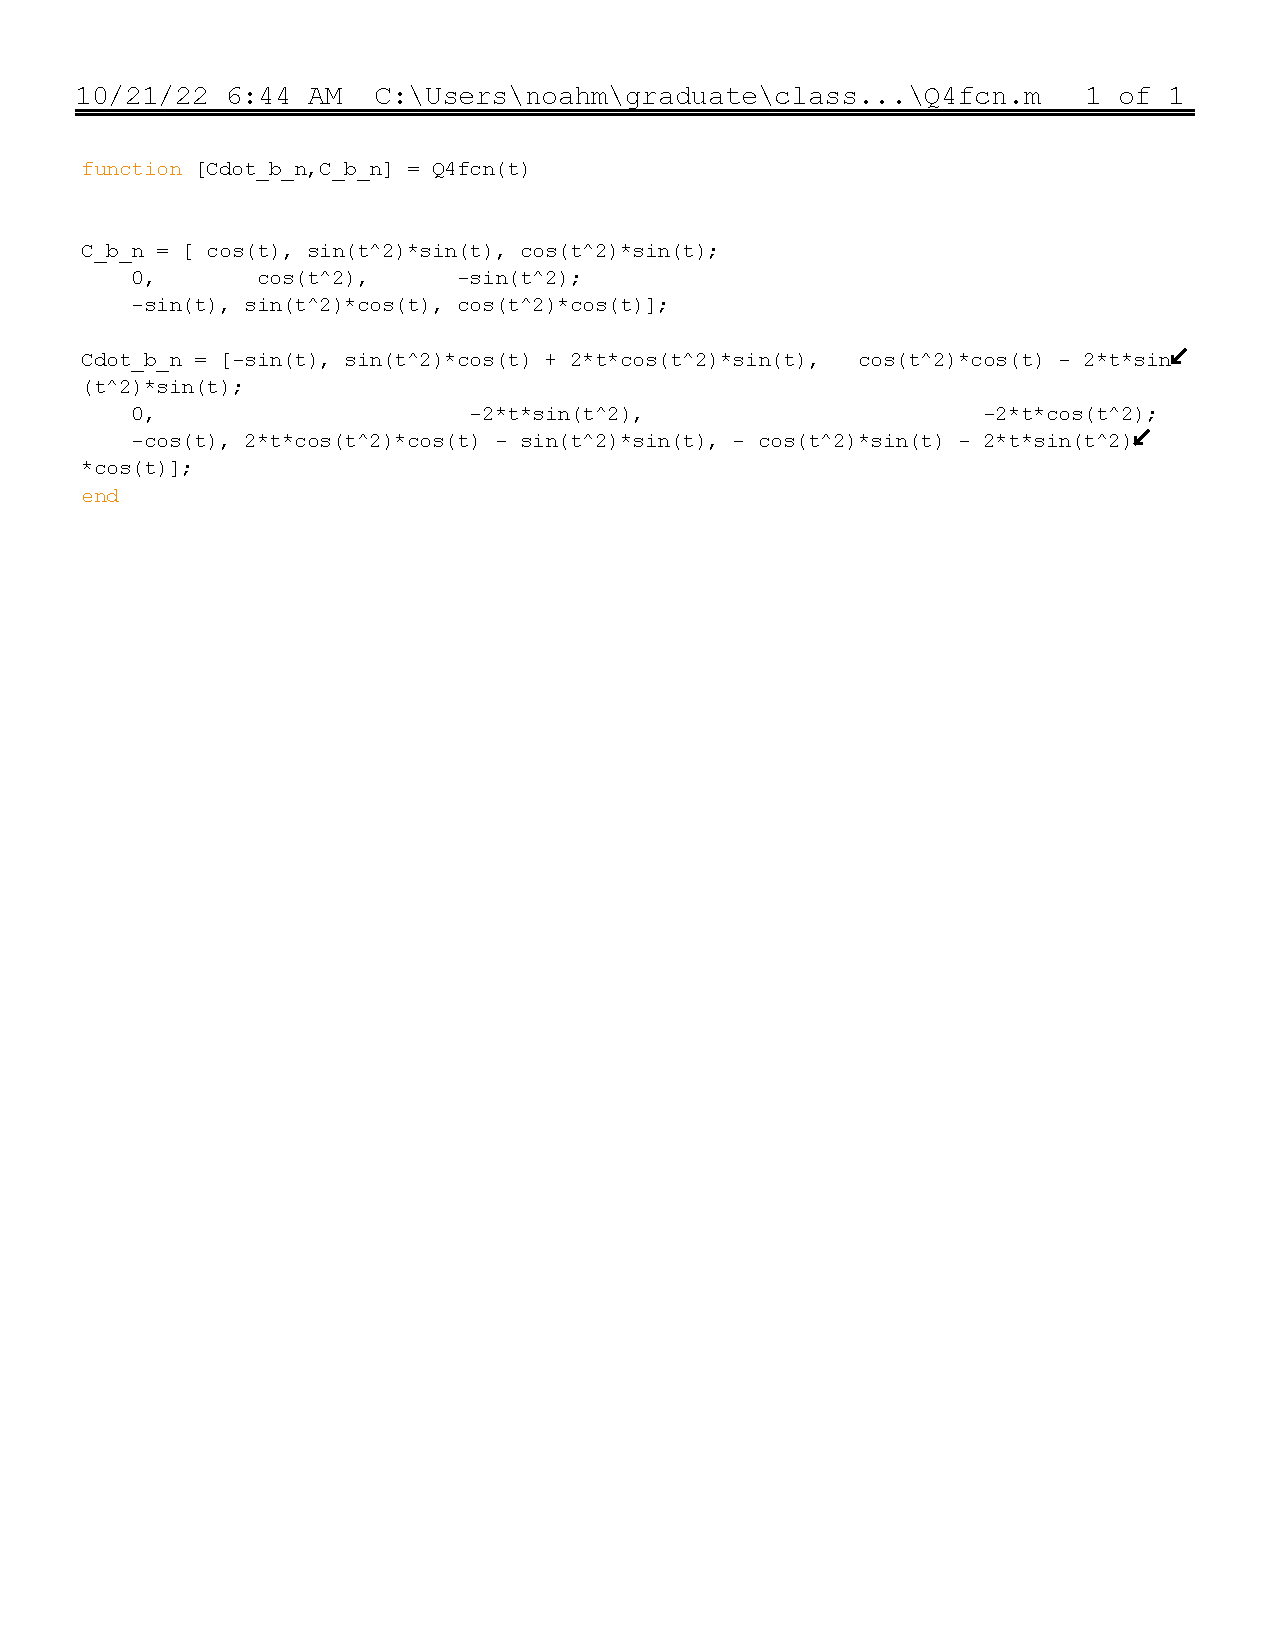
\includepdf[pages={1}]{Q4fcn.pdf}
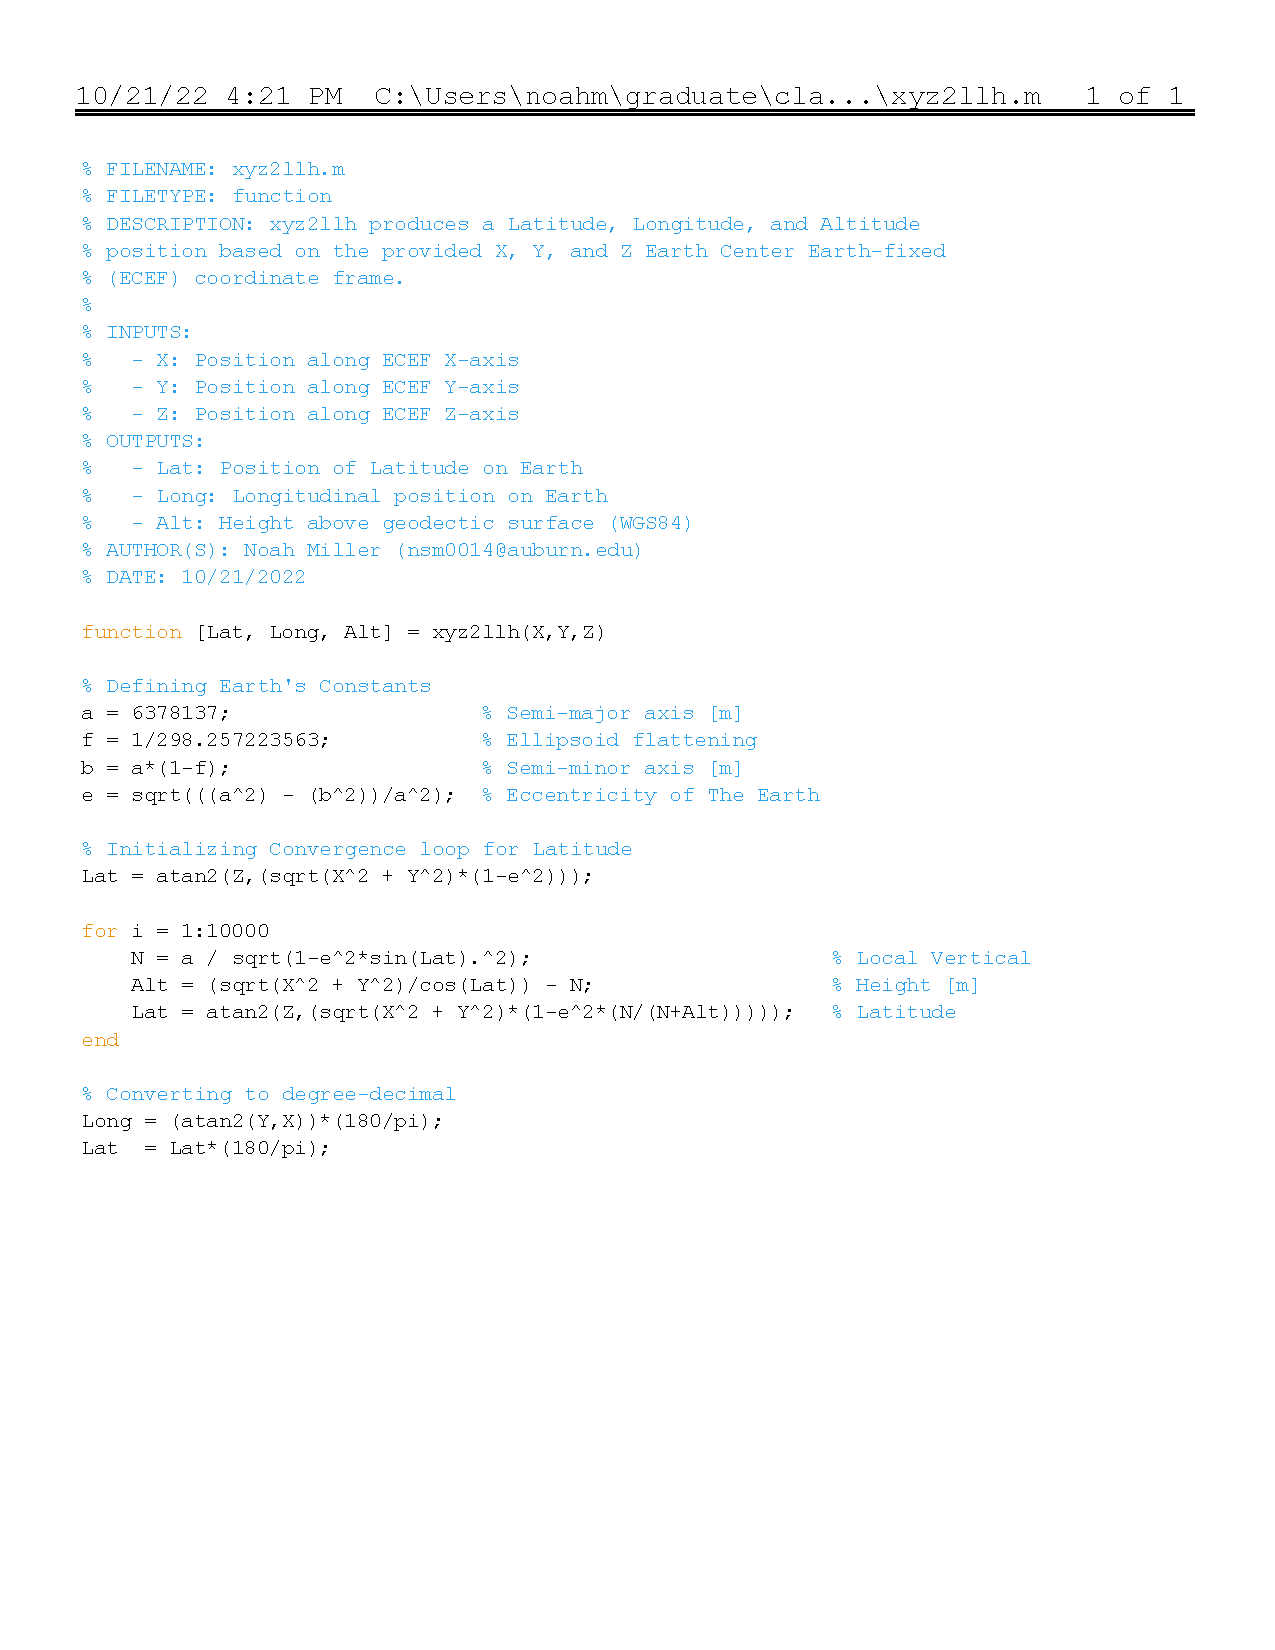
\includepdf[pages={1}]{xyz2llh.pdf}
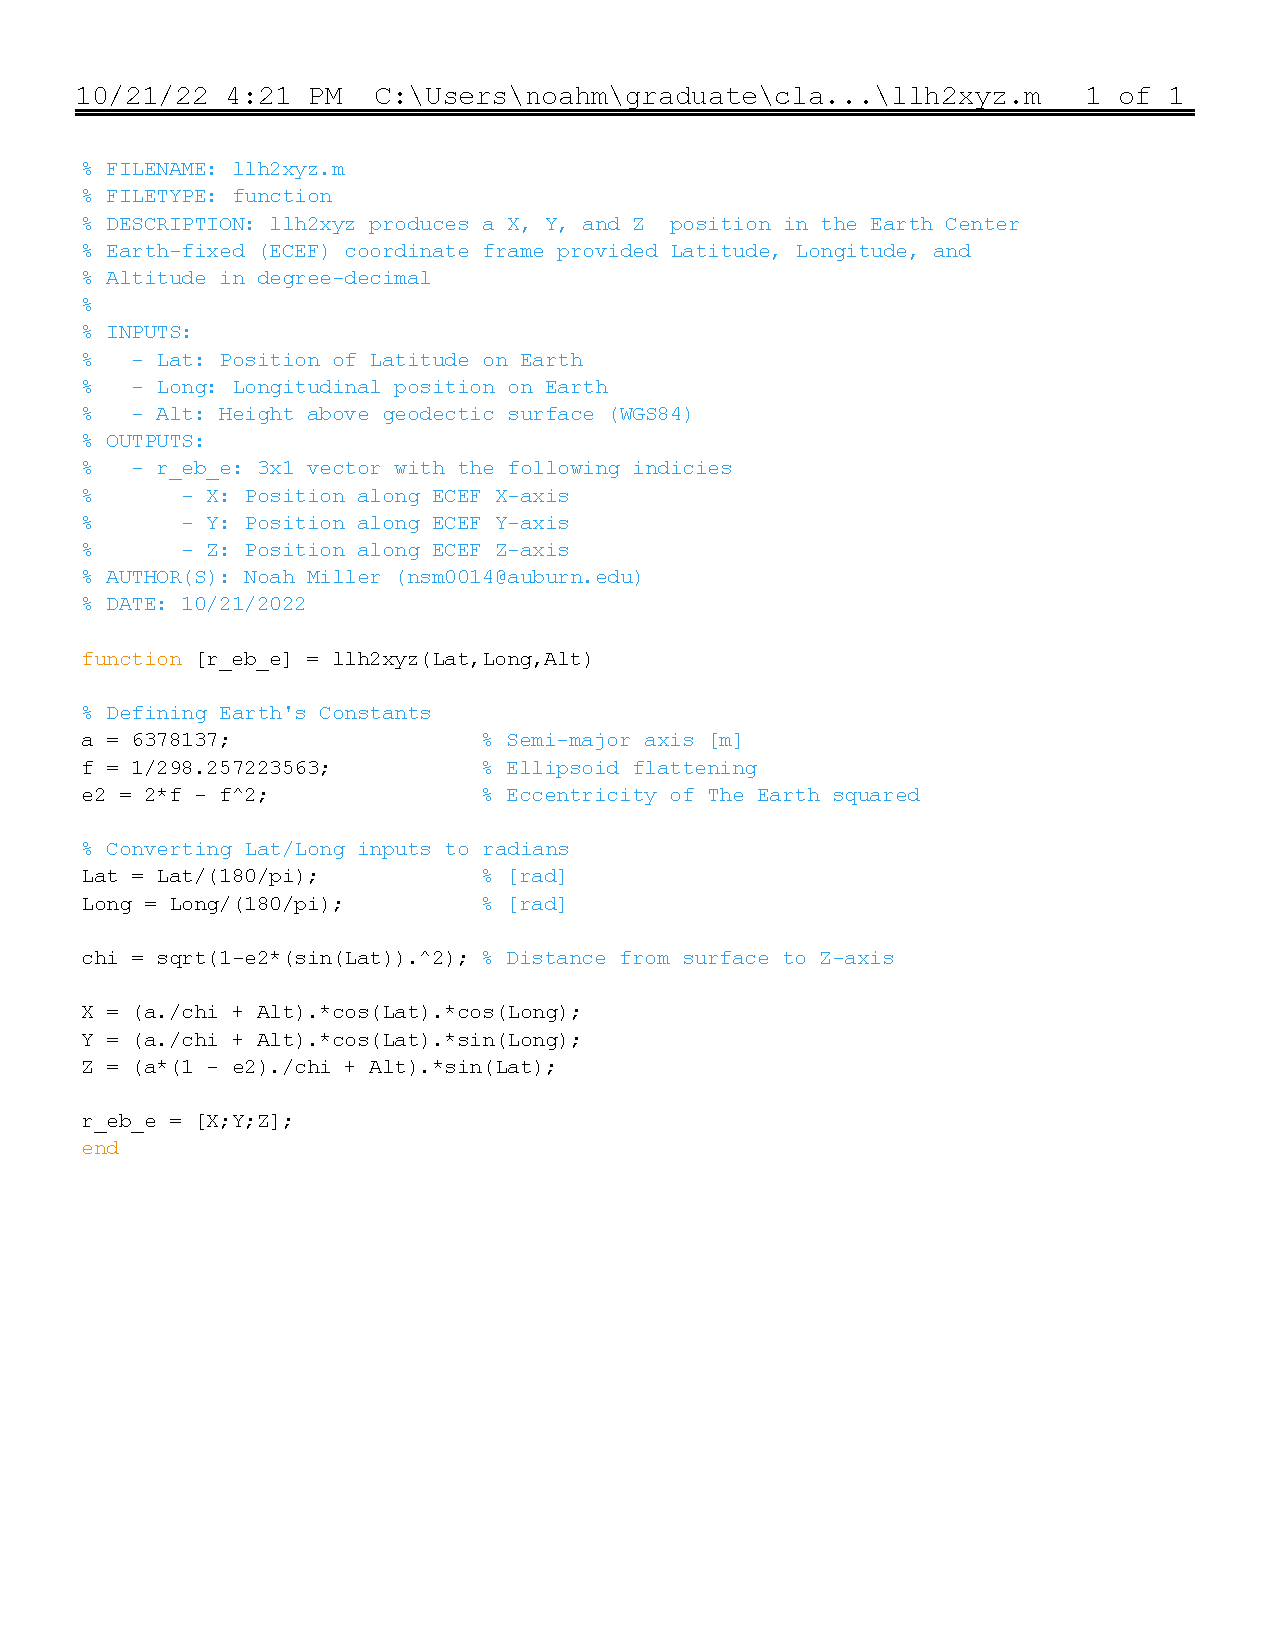
\includepdf[pages={1}]{llh2xyz.pdf}
\includepdf[pages={5-9}]{Hw_3.pdf}

\end{document}